\addcontentsline{toc}{chapter}{Messdaten}
\label{Protokoll}

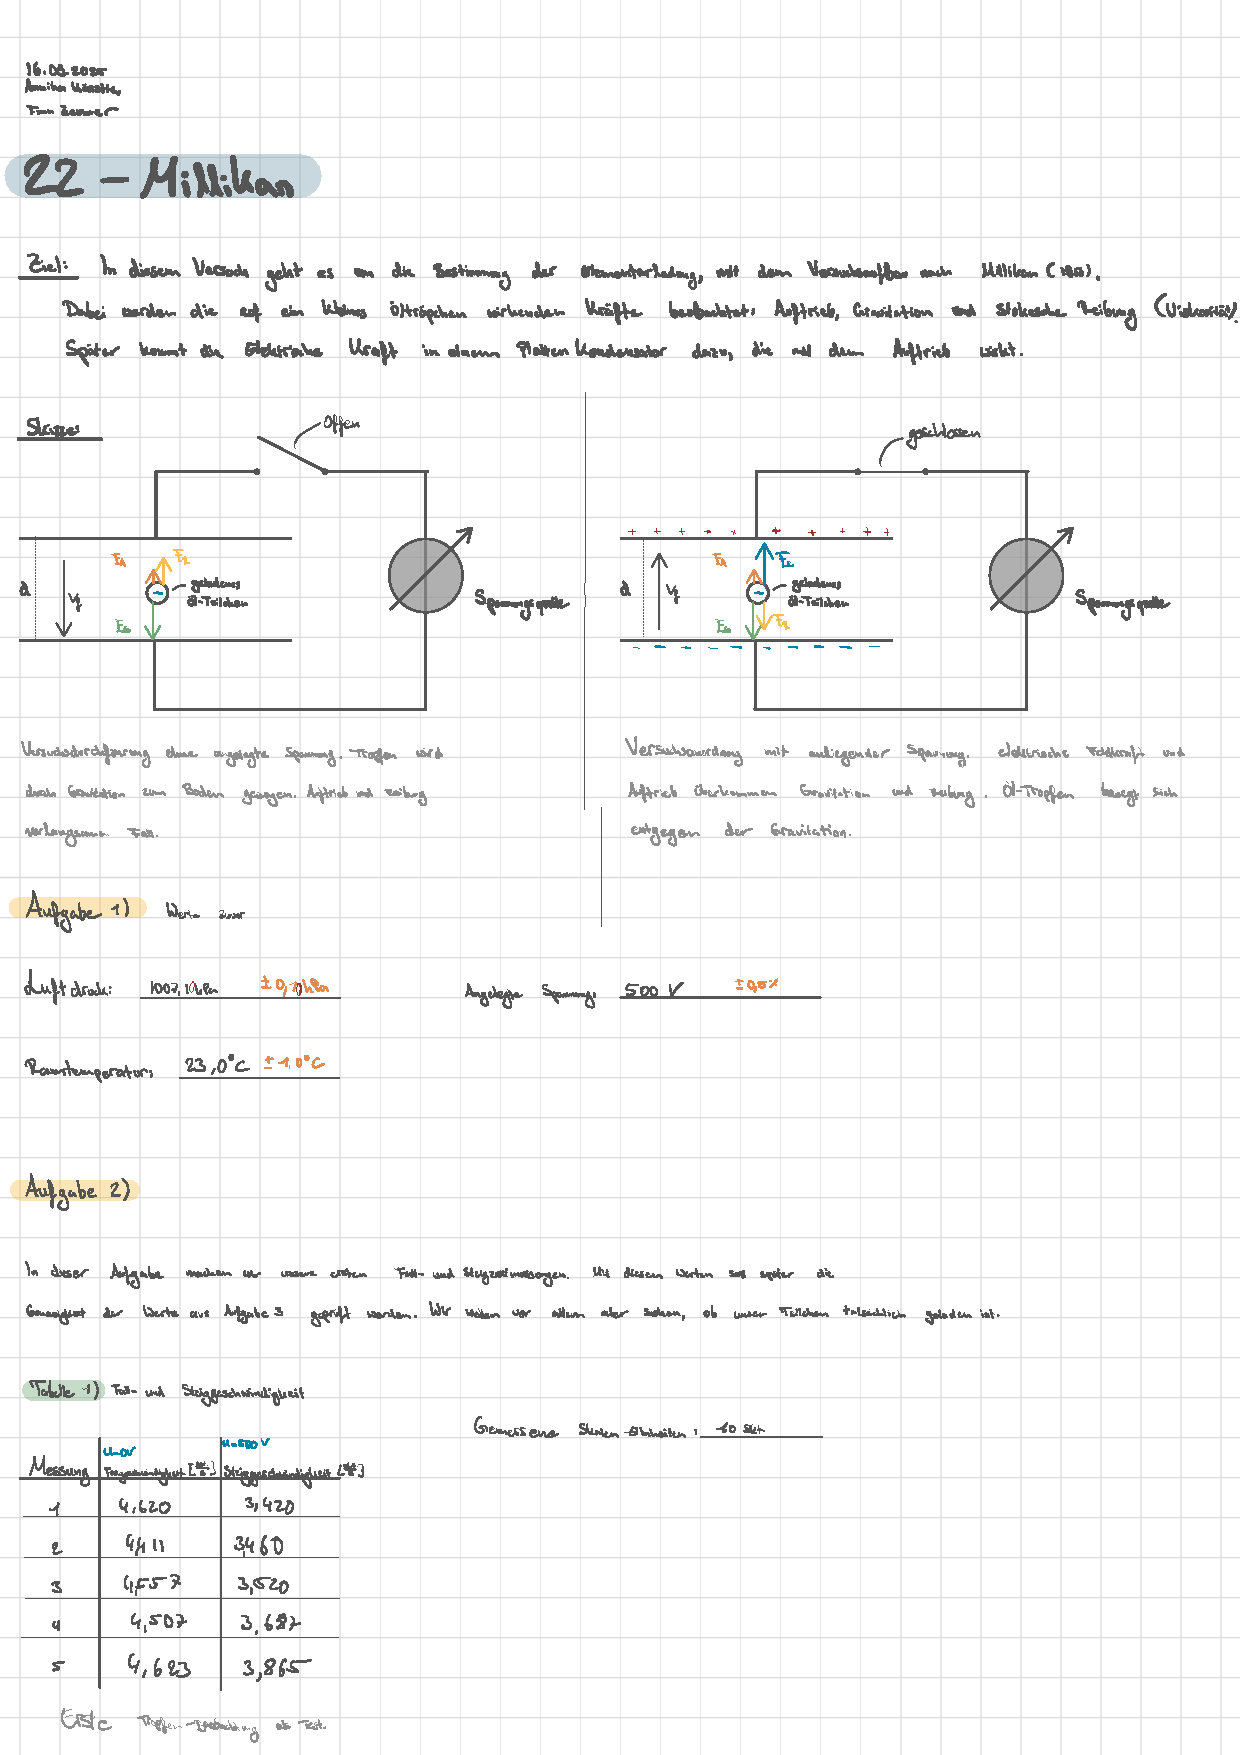
\includepdf[
  pages=1-2,               
  pagecommand={\thispagestyle{empty}} 
]{Protokolle/\versuchsnummer/Chapter/Messprotokoll.pdf}


\addcontentsline{lot}{table}{\protect\numberline{\thechapter.1} Zylinder-Eigenschaften}
\addcontentsline{lot}{table}{\protect\numberline{\thechapter.2} Lichtschrankenabstand}
\addcontentsline{lot}{table}{\protect\numberline{\thechapter.3} Messungen von 4 Zeiten über die schräge Fläche}
\addcontentsline{lot}{table}{\protect\numberline{\thechapter.4} Messung der Zeiten auf der Ebene}
